
\newcommand{\figWidth}{0.24\textwidth}
\begin{figure*}[ht!]
%
% \begin{center}
% \centering
\begin{subfigure}[t]{\figWidth}
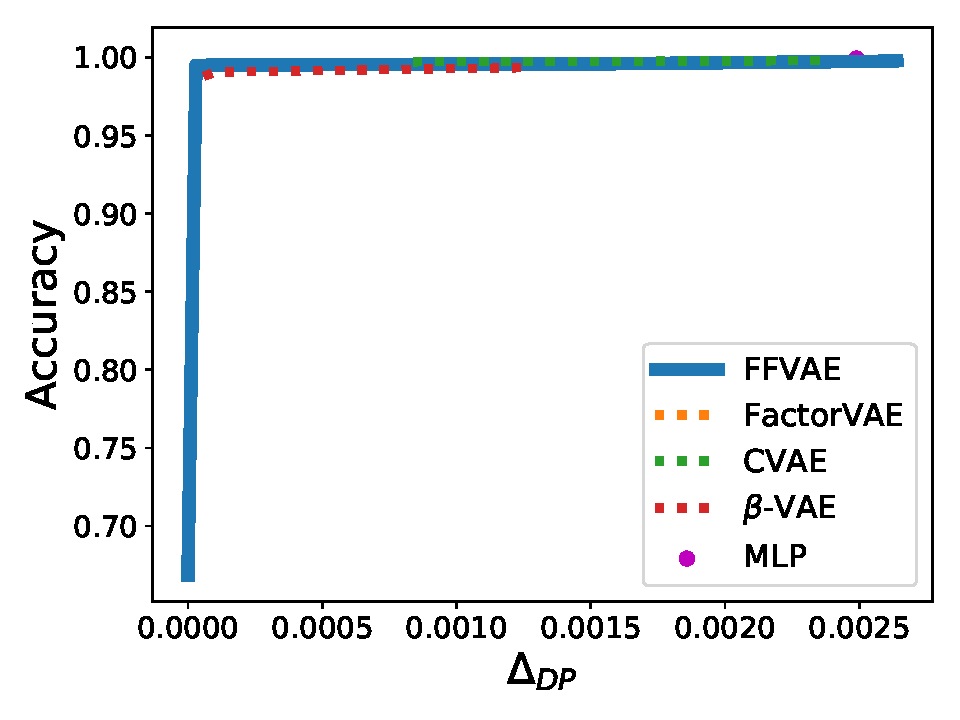
\includegraphics[width=\textwidth]{attr_fn_2_label_fn_4.pdf}
\caption{$a$ = Scale}
\label{fig:dsprites-pareto-a2-y4}
\end{subfigure}
%
\hfill
%
\begin{subfigure}[t]{\figWidth}
% \centering
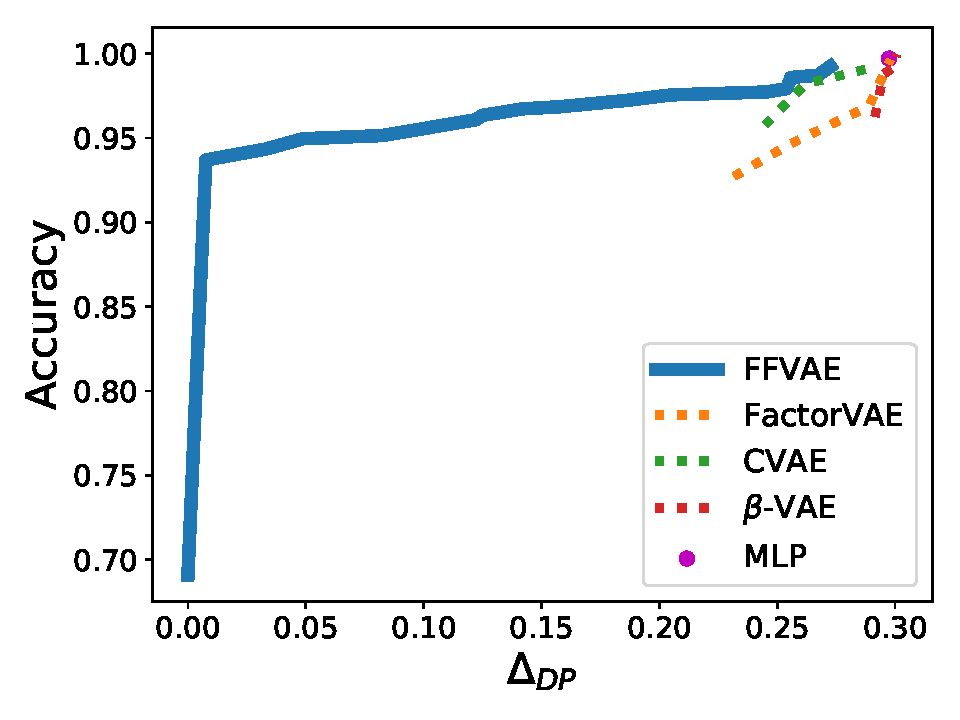
\includegraphics[width=\textwidth]{attr_fn_1_label_fn_4.pdf}
\caption{$a$ = Shape}
\label{fig:dsprites-pareto-a1-y4}
\end{subfigure}
%
\hfill
%
\begin{subfigure}[t]{\figWidth}
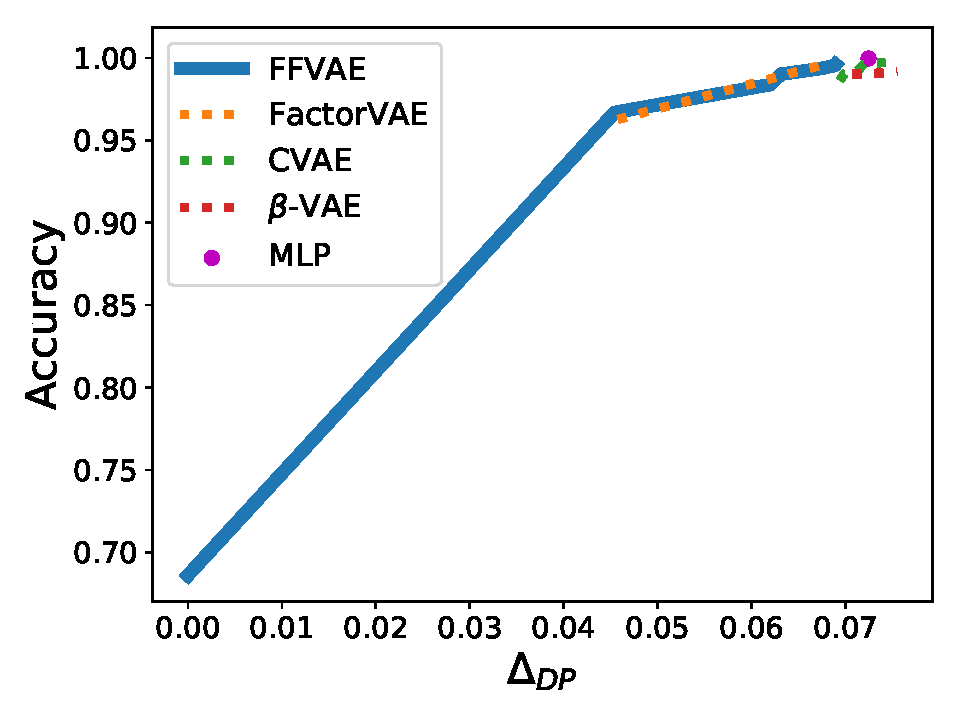
\includegraphics[width=\textwidth]{attr_fn_1_AND_attr_fn_2_label_fn_4.pdf}    
\caption{$a$ = Shape $\wedge$ Scale}
\label{fig:dsprites-pareto-a1and2-y4}
\end{subfigure}
%
\hfill
%
\begin{subfigure}[t]{\figWidth}
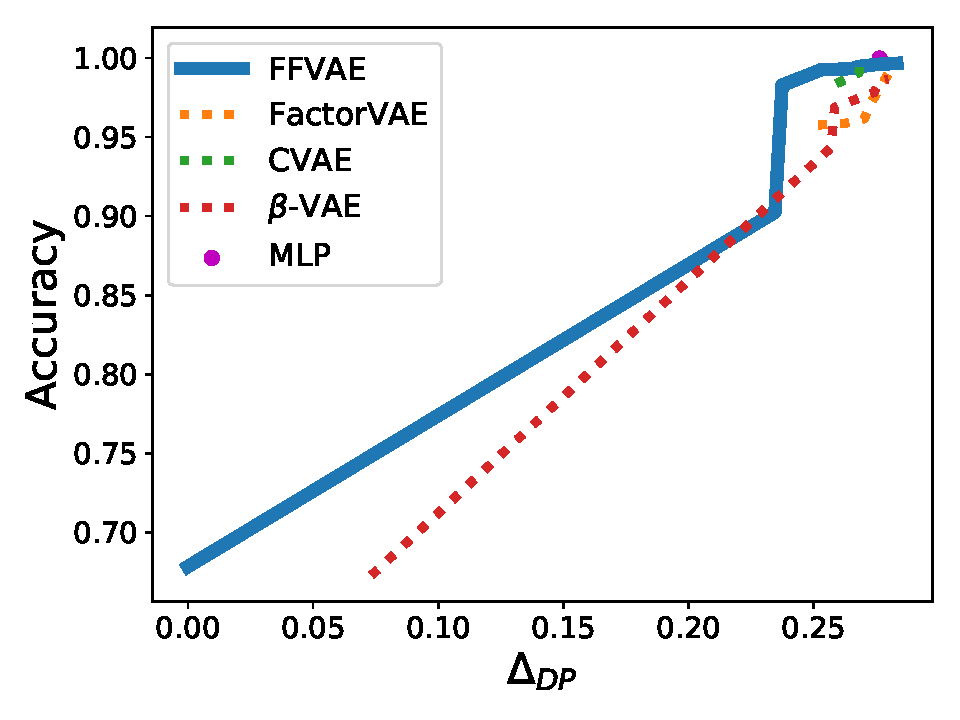
\includegraphics[width=\textwidth]{attr_fn_1_OR_attr_fn_2_label_fn_4.pdf}
\caption{$a$ = Shape $\vee$ Scale}
\label{fig:dsprites-pareto-a1or2-y4}
\end{subfigure}

\caption{
    Fairness-accuracy tradeoff curves, DSpritesUnfair dataset.
    We sweep a range of hyperparameters for each model and report Pareto fronts.
    Optimal point is the top left hand corner --- this represents perfect accuracy and fairness.
    MLP is a baseline classifier trained directly on the input data.
    For each model, encoder outputs are modified to remove information about $a$.
    $y$ = XPosition for each plot.
    }
    \label{fig:dsprites-pareto}
% \end{center}
% \vskip -0.2in
\end{figure*}
